\documentclass[a4paper]{article}
\usepackage{amsmath}
\usepackage{graphicx}
\usepackage{color}
\usepackage{multicol}
\usepackage{float}
 \usepackage{nopageno}
 \usepackage[a4paper]{geometry}
 \usepackage{subfigure}

\begin{document}
\title{\textbf{Coding report}}
\author{Lennie de Roo and Kenneth Elgin, \\
 \emph{Delft University of Technology}}
\date{\normalsize{May, 2015}}
\maketitle 
\noindent \hrulefill
\renewcommand{\abstractname}{}
\begin{abstract}
\noindent This report details a python code that simulates the flow of fluid in a 2D pipe using the D2Q9 Lattice Boltzmann method. The code takes multiple inputs such as relax time and block position and gives graphs for velocity profiles of the pipe as a whole and for a specific slice of the pipe.
\end{abstract}
\hrulefill
\begin{multicols*}{2}
\subsection*{Input}
In the main.py file, \emph{Nxgrid} and \emph{Nygrid} specify the size of the pipe, specifically how many points the pipe consists of in respectively the x- and y-direction. \emph{Dens} determines the total density per point, \emph{timesteps} the number of steps the simulation will run, \emph{pressgradvel} determines how much velocity is added in the x-direction because of the pressure flow in the pipe and \emph{relaxt} is the relaxation time. Taking a higher value for the relaxation time can be useful when one chooses a combination of time steps and pressure gradient value that leads to a turbulent flow in the pipe. The arrays \emph{blocks} and \emph{bigblocks} allow us to respectively create 1-by-1 and n-by-m sized cubes. In the case of \emph{blocks} this is done by adding a value to the array with [xpos,ypos] and for \emph{bigblocks} we use [xstart,xend,ystart,yend]. Lastly, the specific slice of tube that is plotted can be determined using the first component of \emph{velocity} in line 21 of main.py.
\subsection*{Simulation in the code}
The Lattice Boltzmann method is implemented in the code in a step-by-step procedure. First, the grid is initialized by evenly spreading the density given as an input between all 9 directions, while the density inside the blocks is set to 0. Next, the densities are moved using the \emph{numpy roll} command. Once the fluid reaches the end of the pipe in the x-direction, it is reinserted at the other side of the pipe.  On the boundaries and inside the blocks, all directions are flipped according to the bounce back boundary conditions for the Lattice Boltzmann method. Then, the velocity is calculated in both x and y for every point in the grid and it is ensured that the velocity inside the blocks is 0. After this, an additional value is added to the velocity in x-direction. This velocity is then used to calculate the equilibrium density. This is done by calculating the dot product between the e-vector (which describes which direction each of the 9 density groups has) and the velocity as well as dot product of the velocity with itself. Lastly the grid is relaxed using the normal and relaxed density grids and the standard formula for a D2Q9 Lattice Boltzmann grid which calculates the new grid using these two.
\subsection*{Output}
The code outputs a plot of the velocity in x-direction after the given amount of time steps as figure 1. What slice is used can be defined by the user. It also shows a full velocity profile of the complete grid as figure 2. An example of these plots can be seen in figure \ref{fig:plots} in this report. 
 \begin{figure*}
\centering
\subfigure[The velocity profile at x-position 50.]{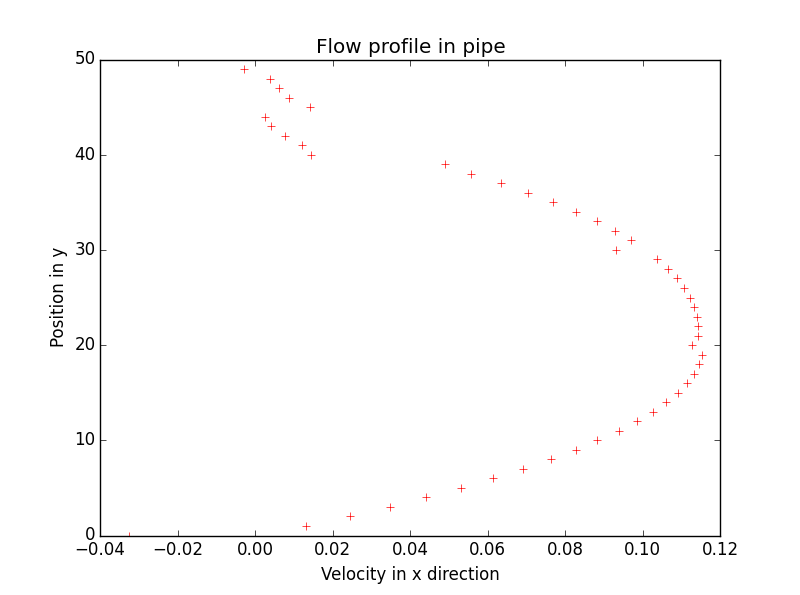
\includegraphics[width=7cm]{velocityplot.png}}
\subfigure[The velocity profile of the complete grid. ]{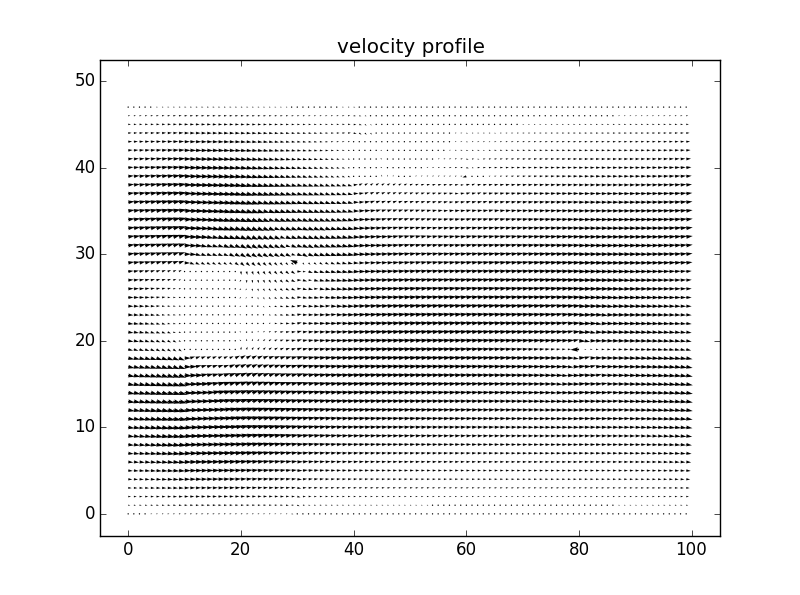
\includegraphics[width=7cm]{quiverplot}}
\caption{The two plots which are outputted by the simulation. In this run a 1000 timesteps were done, the pressure gradient was \emph{pressgradvel=0.005} and the relaxation time \emph{relaxt=4.2 }. There were three blocks of size 1 inserted, and two bigger blocks.}
 \label{fig:plots}
\end{figure*} 
\subsection*{Appendix}
The code for this simulation can be found at github.com/lenniederoo/iccp-flow, with the relevant files being:
\begin{itemize}
\item main.py
\item lattice.py
\end{itemize}
\end{multicols*}
\end{document}